\documentclass{article}

\usepackage[final]{caisc_2026}
\usepackage[utf8]{inputenc}
\usepackage[T1]{fontenc}
\usepackage{hyperref}
\usepackage{url}
\usepackage{booktabs}
\usepackage{graphicx}
\usepackage{amsmath}
\usepackage{microtype}
\usepackage{xcolor}
\usepackage{placeins}
\usepackage{float}

\definecolor{paperblue}{HTML}{2166AC}
\definecolor{paperred}{HTML}{B2182B}
\definecolor{papergray}{HTML}{4D4D4D}
\hypersetup{colorlinks=true,linkcolor=paperred,citecolor=paperblue,urlcolor=paperblue}

\title{When Interface Formatting Changes Model Decisions}

\author{Shailesh Rana\\Independent Researcher}

\begin{document}
\maketitle

\begin{abstract}
Language models increasingly receive the same information through different interfaces: forms, tables, configuration files, markup, and tool-generated records. We ask whether these wrappers are passive containers. We render 3,000 MMLU questions through eight wrappers intended to preserve the question and answer choices, and evaluate Qwen2.5-1.5B, Phi-3.5-mini, and Mistral-7B. The same question crosses the correct--incorrect boundary across wrappers for 62.0\%, 55.1\%, and 66.2\% of items, respectively. Removing audited formatting defects leaves the result essentially unchanged.

Uncertainty predicts some instability but does not explain it. In controlled tests, moving answer content between positions or rotating its displayed A/B/C/D label significantly reduces accuracy in every model, including within every confidence group. We then project intermediate model states into answer-letter and candidate-text scores. At the shared \texttt{Answer:} state, Mistral shows strong evidence consistent with comparatively stable candidate evidence and later output-binding disruption; Phi shows a weaker, instruction-dependent version of this pattern. Qwen's clean first-token result reverses, so its logit lens does not support the same account. The same outward failure therefore need not have one universal internal cause. The combined evidence is consistent with wrapper sensitivity appearing during answer formation, output binding, or both, with the visible pattern depending on the model.
\end{abstract}

\section{Introduction}

A question does not change meaning merely because it is placed in CSV rather than HTML. A reliable model should therefore preserve its answer when the question, candidates, and intended labels remain the same. The tested models often do not. Across eight wrappers, more than half of the questions receive both a correct and an incorrect answer from every model family we test.

This is more than a small change in average accuracy. It is an item-level reliability failure: the same underlying content produces conflicting decisions. Our main question is therefore not only \emph{whether} wrappers matter, but \emph{where} they enter the decision process.

We separate two possibilities:
\begin{enumerate}
    \item \textbf{Answer formation:} the wrapper changes which candidate content the model prefers.
    \item \textbf{Output binding:} useful candidate evidence survives, but the model mishandles its position, displayed label, or required output symbol.
\end{enumerate}
These possibilities can coexist. ``Binding'' here simply means connecting an answer such as \emph{Berlin} to its position and then to the required symbol, such as B.

We build the argument in three steps. First, a behavioral census establishes the wrapper effect across three models. Second, controlled position and label rotations show that binding coordinates causally affect decisions. Third, a layerwise \emph{logit lens}---the model's own output head applied to intermediate states---compares candidate-text and A/B/C/D preferences through depth. The internal result is descriptive rather than causal, but it narrows the explanation: Mistral and Phi are consistent with late output-binding disruption, while Qwen prevents a universal two-stage story.

Our contributions are:
\begin{itemize}
    \item a source-bound, audited evaluation of 72,000 wrapped prompts;
    \item controlled evidence that answer position and displayed labels affect all three models;
    \item a training-free, multi-token-aware logit-lens comparison of candidate and letter trajectories; and
    \item a bounded conclusion: wrapper failures are multi-stage and model-dependent, not evidence for one universal circuit.
\end{itemize}

\section{Related Work}

Prompt sensitivity is well established. Content-free calibration can reduce label bias from prompt format and demonstration order \citep{zhao2021calibrate}. Meaning-preserving prompt formats can produce large performance differences \citep{sclar2024promptformatting}, and evaluating several prompts can change both reported performance and model rankings \citep{mizrahi2024multiprompt}. We focus specifically on structured interface wrappers, bind every analyzed row to stored prompt text, and audit departures from the intended content-preserving contract.

Multiple-choice evaluation also has binding sensitivities. Reordering options can change predictions, especially when a model is uncertain \citep{pezeshkpour2024optionorder}; position shuffles and label replacements can also reduce answer consistency \citep{zhou2024selfconsistency}. Broader studies find sensitivity to both option order and the tokens used to name options \citep{wei2024selectionbias}, while changing only the option-symbol set can materially change accuracy \citep{yang2025optionsymbol}. We therefore treat candidate content, physical position, and displayed label as different variables.

Scoring answer text creates a separate problem: several valid surface forms can compete for probability mass even when they express the same underlying answer \citep{holtzman2021surfaceform}. Our candidate lens avoids open-ended paraphrases and scores only the exact audited candidate strings. This makes the estimand reproducible, but also limits it to those displayed surfaces.

Finally, a standard logit lens need not faithfully expose what intermediate states ``mean'' because those states were not trained to be read directly by the final output head \citep{belrose2023tunedlens}. We use it only to compare predeclared trajectories. We do not treat it as literal access to thought or as proof that the exposed signal controls behavior.

\section{Experimental Design}

\subsection{Questions, wrappers, and models}

We evaluate 3,000 MMLU test questions \citep{hendrycks2021mmlu}. Each has one question, four candidate answers, and one correct candidate. We render each item in eight structured wrappers: CSV, GraphQL, HTML, INI, key--value text, Protocol Buffers, shell heredoc, and TOML. The intended transformation changes syntax and layout while preserving the question, candidate texts, order, and A/B/C/D labels.

We test \texttt{Qwen/Qwen2.5-1.5B-Instruct} \citep{qwen2025qwen25}, \texttt{microsoft/Phi-3.5-mini-instruct} \citep{microsoft2024phi35}, and \texttt{mistralai/Mistral-7B-Instruct-v0.3} \citep{mistralai2024mistral7bv03}. For every prompt, we directly score the next-token likelihood of A, B, C, and D. We do not depend on generated explanations.

Some wrappers favor a letter even when no question is present. We measure this formatting bias with a content-free version of the same wrapper and subtract it from the four letter scores. This is \emph{content-free calibration}. An item is a \emph{wrapper conflict} when at least one wrapper is answered correctly and at least one is answered incorrectly.

\subsection{Audit and protected split}

An outcome-blind audit found 107 content-changing rows and four ambiguous rows among the 24,000 unique item--wrapper prompts. Removing these 111 rows leaves all 3,000 questions represented. We report both the complete census and this audit-adjusted sensitivity analysis.

Mechanistic follow-up uses 2,401 questions: 1,801 discovery-training items and 600 validation items. These names come from the existing artifact split; the logit lens itself trains nothing and pools them only for its predeclared descriptive estimate. The remaining 599 final questions were not opened for intervention design, logit-lens analysis, threshold choice, or reporting.

\subsection{Controlled position and label tests}

We start from the same authenticated prompts and change one binding coordinate at a time:
\begin{itemize}
    \item \textbf{Position rotation:} move candidate content to another physical option position while tracking the same candidate identity.
    \item \textbf{Label rotation:} change which displayed letter names each candidate, again tracking candidate identity.
\end{itemize}
If accuracy falls, the changed coordinate has a causal effect on the model's decision in this controlled setting. This does not by itself show that wrappers amplify the effect.

\subsection{Layerwise candidate and letter readouts}

The logit-lens experiment uses two matched prompt instructions. The \emph{letter contract} asks for only A/B/C/D. The \emph{text contract} changes only that terminal instruction and asks for the actual answer text. For each contract, we measure two readouts at every transformer block:
\begin{enumerate}
    \item \textbf{Letter readout.} Apply the model's final normalization and output head to the hidden state at the last token of the exact \texttt{Answer:} prefix. Score A/B/C/D, then map each displayed letter back to the corresponding candidate identity.
    \item \textbf{Candidate readout.} Score each exact audited candidate continuation in the same tokenizer context. The first candidate token is scored directly from the shared \texttt{Answer:} state. If a candidate contains several tokens, later tokens are teacher-forced and their log-probabilities are added.
\end{enumerate}

For candidate tokens $c_1,\ldots,c_m$ at layer $l$, the full path score is
\begin{equation}
S_l(c)=\sum_{t=1}^{m}\log p_l(c_t\mid \text{prompt},c_{<t}).
\end{equation}
The first term is a clean readout of the shared answer-prefix state. The full sum instead measures how compatible the complete continuation is after supplying each earlier candidate token. It must not be described as information entirely present before generation. We therefore treat the first-token result as the clearest root-state diagnostic and the full path as secondary compatibility evidence. Exact candidate surfaces are used: no synonyms, case variants, optional punctuation, or partial-token matches are added. Duplicate answers, prefix collisions, malformed candidates, and non-unique first tokens remain counted but are excluded from identity comparisons where the comparison would be ambiguous.

At the final block, the lens must reproduce the model's ordinary same-forward-pass A/B/C/D scores within 0.02 log-probability units. Cached-versus-uncached and batched-versus-scalar differences are required to be finite and are recorded; no separate acceptance threshold was tuned for them. Ties are retained as sets rather than broken by option order.

\subsection{Trajectory summary and statistics}

For each layer, we ask whether the plain and wrapped prompts prefer the same candidate. We first average across the eight wrappers within an item and then across items, so one question---not one wrapper row---is the statistical unit. The trajectory summary is the area under this layerwise agreement curve (AUC) over pre-final layers. The main contrast is candidate agreement AUC minus mapped-letter agreement AUC. A positive value means the candidate readout is more stable across wrappers; a negative value means the letter readout is more stable.

Confidence intervals come from item-clustered bootstrap resampling: 2,000 draws for the causal rotations and 5,000 draws for the logit lens, both with seed 1729. The two predeclared full-path contract contrasts receive Holm correction. Layerwise bands are simultaneous; we do not select a favorable layer after seeing the result. The behavioral rates are complete-sample descriptive counts rather than estimates from a random model sample.

\section{Results}

\subsection{Wrappers frequently change answers}

Table~\ref{tab:behavior} shows the central behavioral result. Qwen, Phi, and Mistral answer 62.0\%, 55.1\%, and 66.2\% of questions both correctly and incorrectly across the eight wrappers. The audit-adjusted rates are 61.5\%, 54.8\%, and 66.1\%. The small set of defective rows therefore does not explain the phenomenon.

\begin{table}[H]
\caption{Behavior across eight wrappers. Accuracy is the fraction of calibrated-correct prompt rows. Conflict is the fraction of 3,000 questions with both a correct and an incorrect wrapper answer.}
\label{tab:behavior}
\centering
\small
\begin{tabular}{lccc}
\toprule
Model & Accuracy & Conflict & After audit \\
\midrule
Mistral-7B & 50.3\% & 66.2\% & 66.1\% \\
Phi-3.5-mini & 56.8\% & 55.1\% & 54.8\% \\
Qwen2.5-1.5B & 48.4\% & 62.0\% & 61.5\% \\
\bottomrule
\end{tabular}
\end{table}

Uncertain questions change answers more often, but uncertainty is not sufficient: the controlled binding effects below remain negative in every predeclared confidence tercile.

\subsection{Position and displayed labels causally matter}

Moving candidate content reduces calibrated accuracy by 6.87 points for Mistral, 4.27 for Phi, and 7.99 for Qwen (Table~\ref{tab:causal}). Rotating displayed letters reduces it by 6.08, 4.38, and 6.57 points. Every item-clustered 95\% interval excludes zero, and both effects are negative within every confidence tercile.

\begin{table}[H]
\caption{Change in calibrated accuracy under controlled rotations, in percentage points. Parentheses give item-clustered 95\% bootstrap intervals over 2,401 questions.}
\label{tab:causal}
\centering
\small
\begin{tabular}{lcc}
\toprule
Model & Move content & Rotate labels \\
\midrule
Mistral & $-6.87$ $[-7.84,-5.95]$ & $-6.08$ $[-6.88,-5.29]$ \\
Phi & $-4.27$ $[-5.08,-3.43]$ & $-4.38$ $[-5.03,-3.75]$ \\
Qwen & $-7.99$ $[-9.01,-6.98]$ & $-6.57$ $[-7.35,-5.79]$ \\
\bottomrule
\end{tabular}
\end{table}

This establishes a shared vulnerability: decisions depend on where candidate content appears and which symbol names it. It does \emph{not} prove that wrappers uniquely amplify this vulnerability; the separate wrapper-amplification intervals include zero.

\begin{figure*}[t]
\centering
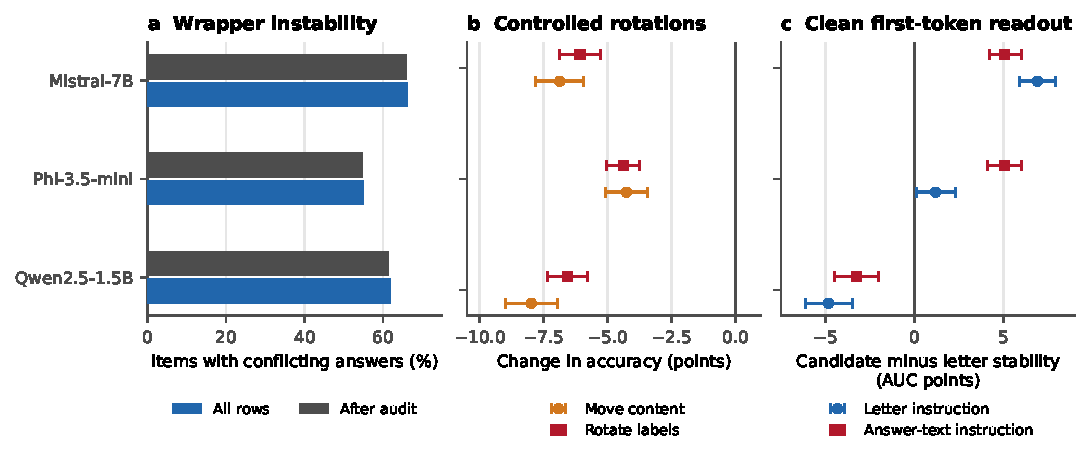
\includegraphics[width=\textwidth]{figures/camera_ready_summary.pdf}
\caption{\textbf{The evidence in one view.} (a) More than half of questions receive conflicting answers across wrappers; the outcome-blind audit barely changes the rates. (b) Controlled position and label rotations reduce accuracy in all models; bars show 95\% item-clustered intervals. (c) At the shared answer-prefix state, first-token candidate preferences are more stable than mapped-letter preferences for Mistral and, under the text instruction, Phi. Qwen reverses. Positive values mean candidate evidence is more wrapper-stable. Legends are placed outside the data regions.}
\label{fig:summary}
\end{figure*}

\subsection{Coarse internal tests did not settle the mechanism}

Earlier diagnostics tested a simpler story: perhaps successful wrappers produce one reusable, wrapper-independent task vector. Coarse attention to the question and candidates barely separated successful from failed wrappers. Successful activations were only slightly closer to the unwrapped prompt. Patching activations from successful presentations produced limited recovery, and in some settings unrelated questions sharing the answer label were better donors than the same question's successful presentation. A candidate-local classifier was also hard to interpret because its target was reconstructed from the emitted letter and its measurement positions were not clean completed-decision states.

These results do not show that candidate evidence is absent. They show that the earlier probes did not isolate a simple reusable state and motivate the cleaner shared \texttt{Answer:} observation used next.

\subsection{The visible internal signature differs by model}

Table~\ref{tab:lens} compares candidate and mapped-letter stability. First-token rows measure the shared answer-prefix state on candidates with distinct first tokens; full paths add teacher-forced tokens.

\begin{table*}[t]
\caption{Candidate agreement AUC minus mapped-letter agreement AUC, in AUC points. Positive values mean candidate preferences are more stable across plain and wrapped prompts. Intervals are 95\% item-clustered bootstrap intervals. Full paths are teacher-forced compatibility scores; first token is the clean shared-state readout.}
\label{tab:lens}
\centering
\small
\begin{tabular}{llrrr}
\toprule
Prompt instruction & Readout & Mistral & Phi & Qwen \\
\midrule
Letter only & First token & $+6.89$ $[5.9,7.9]$ & $+1.18$ $[0.1,2.3]$ & $-4.83$ $[-6.1,-3.5]$ \\
Answer text & First token & $+5.06$ $[4.2,6.0]$ & $+5.04$ $[4.1,6.0]$ & $-3.27$ $[-4.5,-2.0]$ \\
\midrule
Letter only & Full path & $+41.1$ $[40.4,41.8]$ & $+24.0$ $[23.3,24.6]$ & $+36.8$ $[36.0,37.7]$ \\
Answer text & Full path & $+38.4$ $[37.7,39.1]$ & $+30.9$ $[30.3,31.5]$ & $+37.7$ $[36.9,38.5]$ \\
\bottomrule
\end{tabular}
\end{table*}

\paragraph{Mistral.} Candidate first-token preferences are more stable across wrappers than mapped-letter preferences under both instructions: $+6.89$ and $+5.06$ AUC points, with both intervals above zero. Total and token-length-normalized candidate paths agree in direction. This is strong descriptive evidence consistent with comparatively stable answer content and later output-binding disruption.

\paragraph{Phi.} The first-token difference is small under the letter instruction ($+1.18$ points) but larger under the answer-text instruction ($+5.04$). Phi therefore partially reproduces the Mistral pattern, but the strength depends on the requested output. This contract sensitivity matters: changing the output instruction changes the computation, so neither contract is privileged access to a hidden ``true answer.''

\paragraph{Qwen.} Full paths are strongly positive, but the clean first-token contrast reverses under both instructions ($-4.83$ and $-3.27$). Once the first candidate token is supplied, continuing the same candidate becomes easy; this can make full paths look stable without showing that stable candidate evidence was already present at the root. Under the frozen interpretation rule, Qwen's logit lens is therefore \emph{uninformative} about a late-binding mechanism. It is compatible with earlier wrapper-sensitive answer formation, but does not prove it.

The first-token eligible subsets contain 1,008 Mistral items (7,614 wrapped pairs), 1,013 Phi items (7,654 pairs), and 1,042 Qwen items (7,870 pairs). Primary full-path comparisons contain 2,332--2,333 items and 17,626--17,634 pairs, depending on tokenizer eligibility. Train and validation splits reproduce every reported direction. All final-layer parity, finite-value, shape, source-identity, and resume checks pass.

\section{Discussion}

The results support one coherent explanation without forcing one universal circuit:
\begin{quote}
\emph{The evidence is consistent with wrappers interacting with a multi-stage decision process. Sensitivity may appear during candidate formation, output binding, or both, and the visible balance differs by model.}
\end{quote}

The universal result is behavioral and causal. Interface formatting changes decisions, and physical position and displayed labels influence all three models. The internal result is heterogeneous. Mistral gives strong late-binding-consistent evidence; Phi gives weaker, output-instruction-sensitive evidence; Qwen does not support the same account at the clean root measurement. Therefore the paper does not claim that every wrapper failure follows a fixed sequence in which a correct answer is first formed and only later mistranslated into a letter.

Several limits are important. The logit lens applies the final output head to intermediate states that were not trained to be read this way. It is descriptive, not literal access to thought, and it does not establish causal control. Full multi-token paths contain candidate-specific teacher forcing. The first-token analysis is cleaner but covers only candidates with distinguishable first tokens. The study examines three selected instruction-tuned models, one dataset, eight wrappers, and constrained multiple-choice output; models are not a random sample from which to infer a universal population. Finally, wrapper syntax can interact with pretraining associations even when a human judges the content equivalent.

The practical lesson is straightforward. Evaluating one interface is not enough for systems that will receive tables, forms, or tool records. Robustness tests should vary wrapper, candidate position, and output label, and should report item-level conflicts rather than only average accuracy.

\section{Conclusion}

Semantically equivalent interfaces are not computationally equivalent for these language models. Formatting changes answers across three model families, while controlled interventions show that physical position and displayed labels causally affect their decisions. The layerwise evidence does not support assuming one internal route for every failure: Mistral shows a clear late-binding-compatible pattern, Phi partially reproduces it, and Qwen's clean readout reverses.

The final message is simple: interface robustness is not only about whether a model knows an answer. It also depends on how the interface shapes the answer evidence the model forms and how that evidence is connected to the required output.

\paragraph{Code and artifacts.}
The implementation, run cards, tests, compact result tables, and reproduction instructions are available at \url{https://github.com/gut-puncture/interface-formatting-study}.

\bibliographystyle{plainnat}
\bibliography{references}

\section*{Conference For AI Scientists 2026 -- AI Involvement Checklist}

\subsection*{Research Stage Assessment}
\begin{enumerate}
  \item \textbf{Hypothesis development.} Answer: \involvementB{}. Iteration Effort: \iterationMedium{}.

  AI systems proposed candidate hypotheses and experimental designs. The human author selected the research question, bounded the claims, and made the final scientific decisions.

  \item \textbf{Experimental design and implementation.} Answer: \involvementC{}. Iteration Effort: \iterationHigh{}.

  AI coding agents implemented much of the experimental, validation, figure, and packaging pipeline. The human author set the scientific scope, approved interventions, and directed the interpretation safeguards.

  \item \textbf{Analysis of data and interpretation.} Answer: \involvementC{}. Iteration Effort: \iterationHigh{}.

  AI systems computed tables, bootstrap analyses, diagnostics, and draft interpretations. The human author required conservative claim boundaries and made the final interpretation choices.

  \item \textbf{Writing.} Answer: \involvementC{}. Iteration Effort: \iterationHigh{}.

  AI systems drafted and edited the manuscript and figures under detailed human direction. The human author chose the narrative, audience, venue format, and final claims.
\end{enumerate}

\subsection*{AI System Documentation}
\begin{enumerate}
  \setcounter{enumi}{4}
  \item \textbf{AI systems used.} Frontier general-purpose language-model assistants and coding agents with shell execution, data analysis, literature search, and scientific-writing capabilities were used. The experimental subjects are the three open-weight instruction-tuned models named in the paper.

  \item \textbf{Observed AI limitations.} AI systems sometimes over-interpreted weak mechanistic evidence, proposed unnecessary engineering, and drafted conclusions before every numerical receipt was fixed. Source-bound artifacts, automated validation, independent review, and explicit claim limits were needed.
\end{enumerate}

\section*{Conference For AI Scientists 2026 -- Reproducibility and Responsibility Checklist}
\begin{enumerate}
\item \textbf{Claims.} Answer: \answerYes{}. The abstract and introduction state the behavioral, causal, and descriptive internal claims separately.

\item \textbf{Limitations.} Answer: \answerYes{}. The Discussion covers model and dataset scope, tokenizer eligibility, teacher forcing, and the non-causal nature of the logit lens.

\item \textbf{Theory assumptions and proofs.} Answer: \answerNA{}. The paper presents no theoretical theorem.

\item \textbf{Experimental result reproducibility.} Answer: \answerYes{}. Models, prompts, calibration, interventions, splits, observation point, candidate scoring, eligibility, tolerances, statistics, and denominators are disclosed.

\item \textbf{Open access to data and code.} Answer: \answerYes{}. The public repository contains code, tests, run cards, compact artifacts, manifests, and reproduction instructions; model weights and private credentials are excluded.

\item \textbf{Experimental setting/details.} Answer: \answerYes{}. The study performs inference and descriptive analysis, not model training. Runtime settings and exact model revisions are recorded in artifact manifests.

\item \textbf{Experiment statistical significance.} Answer: \answerYes{}. Causal intervals use 2,000 item-cluster bootstrap draws; logit-lens intervals use 5,000 item-cluster draws. The two co-primary full-path contrasts receive Holm correction, and trajectory bands are simultaneous.

\item \textbf{Experiments compute resources.} Answer: \answerYes{}. Hardware model, compute capability, software versions, data type, batching configuration, throughput, and runtime are stored with each run. The new layerwise runs used NVIDIA H200 GPUs; compact outputs omit hidden-state and full-vocabulary tensors.

\item \textbf{Research ethics.} Answer: \answerYes{}. The study uses a public benchmark and open-weight models, with no human subjects or private user data.

\item \textbf{Broader impacts.} Answer: \answerYes{}. Wrapper testing can improve reliability, while the same sensitivity could be used to construct brittle interfaces; both are discussed.
\end{enumerate}

\end{document}
